\documentclass[a4paper]{article}
\usepackage[english]{babel}
\usepackage{amsmath}
\usepackage{amsfonts}
\usepackage{amssymb}
\usepackage{bbold}
\usepackage{graphicx}
\usepackage{blindtext}
\usepackage{hyperref}
\usepackage{mathtools}
\usepackage[export]{adjustbox}

\begin{document}
\pagenumbering{arabic}

\Large
\begin{center}
\textbf{Quantum Fourier Transform}\\
Seminar 2

\hspace{10pt}

\large
BSc. Julio A. Medina$^1$ \\

\hspace{10pt}
\small
$^1$ Universidad de San Carlos, School of Physical and Mathematical Sciences\\
Master's Program in Physics\\
\href{mailto:julioantonio.medina@gmail.com}{julioantonio.medina@gmail.com}\\
\end{center}

\hspace{10pt}

\normalsize
The Fourier transform, and Fourier analysis in general, are ubiquitous mathematical tools in physics. This is expected because many physical phenomena are wave-like in nature; that is, they involve the study of waves in order to be understood. Some important cases in which Fourier analysis is applied in physics include:

\begin{itemize}
\item Quantum mechanics.
\item Seismology.
\item Electromagnetic theory.
\item Mechanical vibrations.
\item Processing of natural and artificial signals.
\item Spectroscopy.
\item Solution of differential equations.
\item Quantum field theory.
\item Quantum computing.
\end{itemize}

\section{Classical Fourier Transform}
\subsection{Fourier Series}
A Fourier series can be defined as an expansion or representation of a function in a series of sines and cosines of the form
\begin{equation}\label{eq::fourier_series}
f(x)=\frac{a_0}{2}+\sum_{n=1}^\infty a_n \cos nx + \sum_{n=1}^\infty b_n \sin nx.
\end{equation}
The conditions imposed on $f(x)$ for the previous equation to be valid are that $f(x)$ must have a finite number of finite discontinuities and a finite number of extrema, maxima and minima. These conditions are known as the Dirichlet conditions. Sturm--Liouville theory (see \cite{Arfken}) guarantees the validity of Eq. \ref{eq::fourier_series}. Using orthogonality relations, the expansion coefficients can be obtained as
\begin{equation*}
a_n=\frac{1}{\pi} \int^{2\pi}_0 f(t) \cos{nt}\, dt
\end{equation*}

\begin{equation*}
b_n=\frac{1}{\pi} \int^{2\pi}_0 f(t) \sin{nt}\, dt, \qquad n=0,1,2,\ldots
\end{equation*}
Substituting the coefficients $a_n$ and $b_n$ into Eq. \ref{eq::fourier_series}, one obtains
\begin{equation}
\begin{aligned}
f(x)&=\frac{1}{2\pi}\int_0^{2\pi} f(t)dt+\frac{1}{\pi}\sum_{n=1}^\infty\Big[ \cos{nx}\int_0^{2\pi} f(t) \cos{nt}\,dt + \sin{nx}\int_0^{2\pi} f(t) \sin{nt}\,dt \Big]\\
&=\frac{1}{2\pi}\int_0^{2\pi} f(t)dt+\frac{1}{\pi}\sum^\infty_{n=1} \int^{2\pi}_0 f(t)\cos{n(x-t)}\,dt.
\end{aligned}
\end{equation}
The previous expressions are valid to represent the function $f(x)$ on the interval $[0,2\pi]$. To represent it on an interval of length $2L$, Eq. \ref{eq::fourier_series} and its coefficients can be written as
\begin{equation}
f(x)=\frac{a_0}{2}+\sum_{n=1}^\infty \Big[ a_n \cos{\frac{n\pi x}{L}} + b_n \sin{\frac{n\pi x}{L}} \Big]
\end{equation}
\begin{equation}\label{eq::Fourier_coeff}
\begin{aligned}
a_n&=\frac{1}{L} \int^{L}_{-L} f(t) \cos{\frac{n\pi t}{L}}\, dt \\
b_n&=\frac{1}{L} \int^{L}_{-L} f(t) \sin{\frac{n\pi t}{L}}\, dt, \qquad n=0,1,2,\ldots
\end{aligned}
\end{equation}

\subsection{Fourier Integral}
As mentioned above, Fourier series are especially useful for representing certain types of functions over a defined range: $[0,2\pi]$, $[-L,L]$, and so on as needed, or over the interval $[-\infty,\infty]$ if the function is periodic. We now analyze the problem of representing a non-periodic function over an infinite range. Physically, this can be interpreted as the decomposition of an isolated pulse or wave packet into its sinusoidal components. The Fourier series coefficients on the interval $[-L,L]$, given by Eq. \ref{eq::Fourier_coeff}, lead to the Fourier series
\begin{equation}
\begin{aligned}
f(x)=\frac{1}{2L}\int^L_{-L} f(t)\,dt + \frac{1}{L}\sum_{n=1}^\infty \cos{\frac{n\pi x}{L}}\int^L_{-L} f(t) \cos{\frac{n\pi t}{L}}\, dt +\\
 \frac{1}{L}\sum_{n=1}^{\infty}\sin{\frac{n \pi x}{L}}\int^L_{-L} f(t) \sin\frac{n\pi t}{L}\,dt.
\end{aligned}
\end{equation}
This can be rewritten as
\begin{equation}
f(x)=\frac{1}{2L}\int^L_{-L} f(t)\, dt + \frac{1}{L}\sum^\infty_{n=1}\int^L_{-L} f(t)\cos\frac{n\pi}{L}(t-x)\,dt.
\end{equation}
Now let the parameter $L$ approach infinity, transforming the finite interval $[-L,L]$ into the infinite interval $(-\infty,\infty)$. Define
\begin{equation}
\omega=\frac{n\pi}{L}, \qquad \Delta\omega=\frac{\pi}{L}, \qquad \text{with } L\rightarrow\infty.
\end{equation}
With this, one obtains
\begin{equation}
f(x)\rightarrow \frac{1}{\pi}\sum_{n=1}^\infty \Delta\omega \int_{-\infty}^\infty f(t) \cos{\omega(t-x)}\,dt,
\end{equation}
and replacing the infinite sum by an integral over $\omega$ gives
\begin{equation}\label{eq::Fourier_integral}
f(x)=\frac{1}{\pi}\int_0^\infty\,d\omega \int_{-\infty}^\infty f(t)\cos{\omega(t-x)}\,dt.
\end{equation}
The $a_0$ term vanishes assuming that $\int_{-\infty}^\infty f(t)\,dt$ exists.

The result in Eq. \ref{eq::Fourier_integral} is known as the Fourier integral. It can be conveniently expressed in exponential form by noting that
\begin{equation}\label{eq::Fourier_cosine}
f(x)=\frac{1}{2\pi}\int_{-\infty}^{\infty}d\omega \int_{-\infty}^\infty f(t) \cos\omega(t-x)\, dt,
\end{equation}
and that
\begin{equation}\label{eq::Fourier_sine}
\frac{1}{2\pi}\int_{-\infty}^\infty d\omega \int_{-\infty}^\infty f(t) \sin\omega(t-x)\, dt=0.
\end{equation}
These results follow from the fact that $\cos \omega(t-x)$ is an even function of $\omega$, while $\sin\omega(t-x)$ is an odd function of $\omega$. Adding Eq. \ref{eq::Fourier_cosine} and Eq. \ref{eq::Fourier_sine} multiplied by the imaginary unit $i$, one obtains
\begin{equation}\label{eq::Fourier_exponetial}
f(x)=\frac{1}{2\pi}\int_{-\infty}^\infty e^{-i \omega x }\,d\omega \int_{-\infty}^\infty f(t)e^{i\omega t}\,dt.
\end{equation}
The variable $\omega$ is an arbitrary variable, also known as a dummy variable. It plays the same role as an index in a summation. However, in many physical problems, $\omega$ represents an angular frequency. Thus, Eqs. \ref{eq::Fourier_cosine} and \ref{eq::Fourier_exponetial} can be interpreted as representations of $f(x)$ in terms of a distribution of infinite wavefronts with angular frequency $\omega$, where the frequency is a continuous real variable.

\subsection{Fourier Transform}
Define a function $g(\omega)$ as the Fourier transform through
\begin{equation}\label{eq::Fourier_transform}
g(\omega)\equiv \frac{1}{\sqrt{2\pi}}\int_{-\infty}^\infty f(t) e ^{i\omega t }\, dt.
\end{equation}
Then it is easy to see from the Fourier integral, Eq. \ref{eq::Fourier_exponetial}, that
\begin{equation}\label{eq::Inverse_Fourier_transform}
f(x)=\frac{1}{\sqrt{2\pi}}\int_{-\infty}^\infty g(\omega)e^{-i \omega x}\, d\omega.
\end{equation}
This relation is also known as the inversion theorem or inverse Fourier transform. It is worth noting that Eqs. \ref{eq::Fourier_transform} and \ref{eq::Inverse_Fourier_transform} are almost symmetric, but they differ in the sign of the imaginary unit $i$.

\section{Quantum Fourier Transform}
\subsection{Introduction}
As mentioned before, the Fourier transform has many applications throughout physics and also has important applications in classical computing, such as signal processing, data compression algorithms, and algorithmic complexity theory. The Quantum Fourier Transform is the quantum implementation of the discrete Fourier transform over the amplitudes of a wave function\footnote{A wave function that evolves according to the Schr\"{o}dinger equation.}. It is a fundamental component of several quantum algorithms, such as Shor's factoring algorithm and quantum phase estimation.

The quantum Fourier transform acts on a vector $(x_0, \ldots, x_{N-1})$ and maps it to another vector $(y_0, \ldots, y_{N-1})$ through the formula
\begin{equation}
y_{k}=\frac{1}{\sqrt{N}}\sum_{j=0}^{N-1}x_j \omega_{N}^{jk}
\end{equation}
where
\begin{equation}\label{eq::omega_definition}
\omega_{N}^{jk}=e^{2\pi i \frac{jk}{N}}.
\end{equation}

Analogously, the quantum Fourier transform acts on a quantum state\footnote{A vector in a finite- or infinite-dimensional Hilbert space.}
\begin{equation}
|X\rangle=\sum_{j=0}^{N-1} x_{j}|j\rangle
\end{equation}
and maps it to the state
\begin{equation}\label{eq::QFT_general}
|Y\rangle=\sum_{k=0}^{N-1} y_{k}|k\rangle
\end{equation}
according to the expression
\begin{equation}
y_k=\frac{1}{\sqrt{N}}\sum_{j=0}^{N-1}x_j\omega_{N}^{jk}
\end{equation}
where $\omega_{N}^{jk}$ is defined in Eq. \ref{eq::omega_definition}. It is important to note that only the amplitudes of the state are affected by this transformation. This can also be expressed as the mapping
\begin{equation}
|j\rangle \rightarrow \frac{1}{\sqrt{N}}\sum^{N-1}_{k=0}\omega_N^{jk}|k\rangle
\end{equation}
or by the unitary matrix
\begin{equation}
U_{\text{QFT}}=\frac{1}{\sqrt{N}}\sum_{j=0}^{N-1}\sum_{k=0}^{N-1}\omega_{N}^{jk}|k\rangle\langle j|.
\end{equation}

\subsubsection{Intuition Behind the QFT}
The intuition behind the Quantum Fourier Transform (QFT) comes from the fact that, when it transforms a quantum state, it essentially changes from the computational $Z$ basis to the Fourier basis. The Hadamard gate (\cite{Medina}, \cite{Qiskit}, \cite{Nielsen}) is the quantum Fourier transform for a single qubit: it transforms from the computational $Z$ basis $\{|0\rangle, |1\rangle\}$ to the $X$ basis $\{|+\rangle, |-\rangle \}$. In the same way, every multi-particle state, that is, every multi-qubit state in the computational basis, has a representation in the Fourier basis. The QFT is simply the function that transforms between these bases.
\begin{equation}
\text{QFT}|x\rangle = |\tilde{x}\rangle,
\end{equation}
where the Fourier basis is denoted by $|\tilde{x}\rangle$.

\subsection{Example 1: One-Qubit QFT}
We begin by considering how the previously defined QFT operator acts on a single-qubit state, i.e. $|\psi\rangle=\alpha|0\rangle+\beta |1\rangle$. For this case, $x_0=\alpha$, $x_1=\beta$, and $N=2$. Therefore, the first Fourier coefficient in the transformation is
\begin{equation}
y_0=\frac{1}{\sqrt{2}}\Bigg( \alpha \exp\bigg( 2\pi i \frac{0\times 0}{2} \bigg) + \beta \exp\bigg( 2\pi i \frac{1\times 0}{2} \bigg) \Bigg)=\frac{1}{\sqrt{2}}(\alpha+\beta)
\end{equation}
and for the second coefficient,
\begin{equation}
y_1=\frac{1}{\sqrt{2}}\Bigg( \alpha \exp\bigg( 2\pi i \frac{0\times 1}{2} \bigg) + \beta \exp\bigg( 2\pi i \frac{1\times 1}{2} \bigg) \Bigg)=\frac{1}{\sqrt{2}}(\alpha-\beta).
\end{equation}
Thus, the total result on $|\psi\rangle$ is
\begin{equation}
U_{\text{QFT}}|\psi\rangle=\frac{1}{\sqrt{2}}(\alpha+\beta)|0\rangle + \frac{1}{\sqrt{2}}(\alpha-\beta)|1\rangle.
\end{equation}
This operation is equivalent to applying the Hadamard operator
\begin{equation}\label{eq::Hadamard_gate}
H=\frac{1}{\sqrt{2}}
\begin{bmatrix}
1&1\\
1&-1
\end{bmatrix}
\end{equation}
to the state $\vert \psi\rangle$,
\begin{equation}
\begin{aligned}
H\vert\psi\rangle&=\frac{1}{\sqrt{2}}(\alpha+\beta)|0\rangle + \frac{1}{\sqrt{2}}(\alpha-\beta)|1\rangle\equiv \tilde{\alpha}\vert 0\rangle+ \tilde{\beta}\vert 1\rangle\\
&=\alpha \vert + \rangle +\beta \vert - \rangle.
\end{aligned}
\end{equation}

\subsection{Quantum Fourier Transform: General Definition}
The previous example does not make completely clear how a quantum Fourier transform is applied for larger $N$. Here, take $N=2^n$, that is, $U_{\text{QFT}_N}$ acts on the state $|x\rangle=|x_1\ldots x_n\rangle$\footnote{We use the notation $|x_1\ldots x_n\rangle=|x_1\rangle\otimes\ldots\otimes |x_n\rangle$.}, where $x_1$ is the most significant bit. Applying Eq. \ref{eq::QFT_general}, one obtains
\begin{equation}\label{eq::QFT}
\begin{aligned}
U_{\text{QFT}_N}|x\rangle &=\frac{1}{\sqrt{N}}\sum_{y=0}^{N-1}\omega_N^{xy}|y\rangle\\
&=\frac{1}{\sqrt{N}}\sum_{y=0}^{N-1} e^{2\pi i xy/2^{n}}|y\rangle.
\end{aligned}
\end{equation}
Rewriting $y$ in binary fractional notation $y=y_1\ldots y_n$ with
\begin{equation*}
\frac{y}{2^n}=\sum_{k=1}^{n}\frac{y_k}{2^k},
\end{equation*}
where $y_k \in\{ 0, 1 \}$, and substituting into Eq. \ref{eq::QFT}, one obtains
\begin{equation}\label{eq::QFT_2}
\begin{aligned}
U_{\text{QFT}_N}|x\rangle &=\frac{1}{\sqrt{N}}\sum_{y=0}^{N-1}e^{2\pi i x(\sum_{k=1}^n y_k/2^k)}|y_1 \ldots y_n\rangle\\
&=\frac{1}{\sqrt{N}}\sum_{y=0}^{N-1} \prod_{k=1}^n e^{2\pi i x y_k/2^{k}}|y_1 \ldots y_n\rangle.
\end{aligned}
\end{equation}
Here, the exponential of a sum has been expressed as a product of exponentials. Rearranging the sums and products, and expanding $\sum_{y=0}^{N-1}=\sum_{y_1=0}^1 \sum_{y_2=0}^1 \ldots \sum_{y_n=0}^1$, gives
\begin{equation}\label{eq::QFT_3}
\begin{aligned}
U_{\text{QFT}_N}|x\rangle &=\frac{1}{\sqrt{N}} \bigotimes_{k=1}^n \bigg(|0\rangle + e^{2\pi i x/2^k}|1\rangle \bigg)  \\
&=\frac{1}{\sqrt{N}}\bigg(|0\rangle + e^{\frac{2\pi i}{2} x} |1\rangle \bigg)\otimes\bigg(|0\rangle + e^{\frac{2\pi i}{2^2} x} |1\rangle \bigg)\otimes \ldots \otimes \bigg(|0\rangle + e^{\frac{2\pi i}{2^{n}} x} |1\rangle \bigg).
\end{aligned}
\end{equation}

\section{Circuit for the Quantum Fourier Transform}
The quantum Fourier transform can be implemented using the quantum circuit model used by several real implementations of quantum computing. For an introduction to these circuits, see \cite{Qiskit}, \cite{Medina}, \cite{Nielsen}, etc. To build the QFT circuit, two gates are used. The first is a single-qubit gate, the Hadamard gate in Eq. \ref{eq::Hadamard_gate}. From the discussion of the one-qubit QFT example and from the derivation of the general expression for the QFT, it is known that, for the single-qubit state $\vert x_k\rangle$, the corresponding quantum Fourier transform is
\begin{equation}
H\vert x_k\rangle=\frac{1}{\sqrt{2}}\bigg(\vert 0\rangle + \exp{\bigg(\frac{2\pi i}{2} x_k\bigg)}\vert 1\rangle\bigg).
\end{equation}
The second two-qubit gate is the controlled rotation $C\,\text{ROT}_k$, which in block-matrix notation is defined as
\begin{equation}
C\,\text{ROT}_k=
\begin{bmatrix}
\mathbf{I}& 0\\
0& U\,\text{ROT}_k\\
\end{bmatrix}
\end{equation}
where
\begin{equation}
U\,\text{ROT}_k=
\begin{bmatrix}
1& 0\\
0& \exp{\big(\frac{2\pi i}{2^k}\big)}\\
\end{bmatrix}.
\end{equation}
The effect of applying $C\,\text{ROT}_k$ to a two-qubit state $\vert x_l x_j\rangle$, where the first qubit is the control qubit and the second qubit is the target, is given by
\begin{equation}
C\,\text{ROT}_k \vert 0\,x_j\rangle=\vert 0 \, x_j\rangle
\end{equation}
and
\begin{equation}
C\,\text{ROT}_k \vert 1\,x_j\rangle=\exp{\bigg(\frac{2\pi i }{2^k} x_j\bigg)}\vert 1 \, x_j\rangle.
\end{equation}
With these two gates, the circuit that implements the quantum Fourier transform can be built as shown in the following diagram.

\begin{figure}[h]
\begin{center}
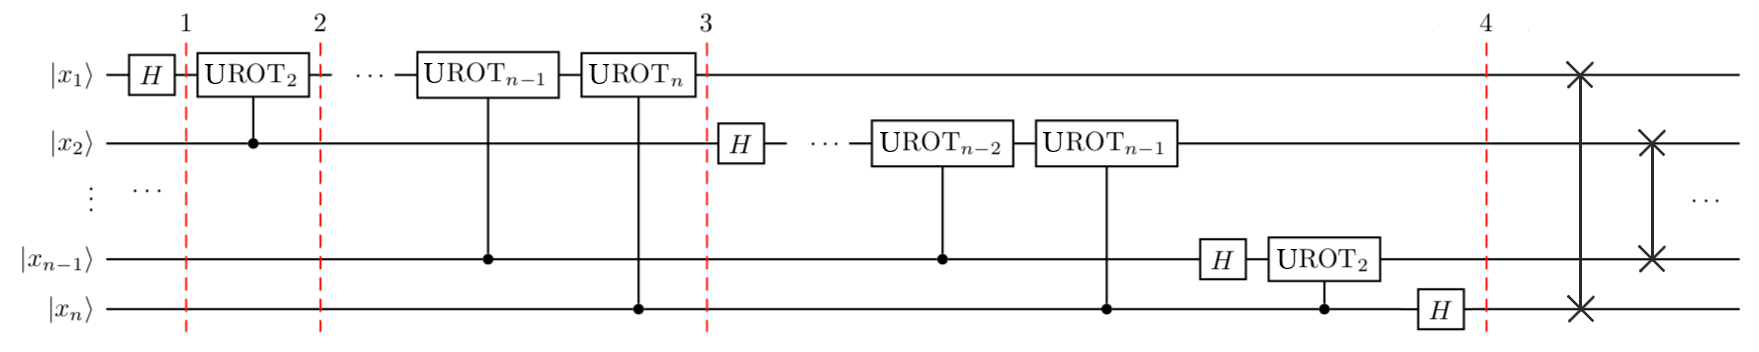
\includegraphics[scale=0.29]{./qft_circuit.png}
\end{center}
\caption{QFT circuit implementation.}
\label{fig::QFT_circuit_general}
\end{figure}

The circuit operates as follows. We start with an input state $\vert x_1\, x_2\ldots x_n\rangle$.
\begin{enumerate}
\item Apply the Hadamard gate to the first qubit, transforming the input state as follows:
\begin{equation}
H_1\vert x_1 x_2\ldots x_n\rangle=\frac{1}{\sqrt{2}}\bigg[\vert 0\rangle + \exp{\bigg(\frac{2\pi i }{2} x_1\bigg)}\vert 1\rangle\bigg] \otimes \vert x_2 x_3\ldots x_n\rangle.
\end{equation}
\item Then apply the $U\,\text{ROT}_2$ gate to qubit 1 controlled by qubit 2. This results in
\begin{equation}
\frac{1}{\sqrt{2}}\bigg[\vert 0\rangle + \exp{\bigg(\frac{2\pi i }{2^2} x_2+\frac{2\pi i }{2} x_1\bigg)}\vert 1\rangle\bigg] \otimes \vert x_2 x_3\ldots x_n\rangle.
\end{equation}
\item This process is repeated until qubit $n$ is reached. That is, when the last gate $U\,\text{ROT}_n$ is applied to qubit 1 controlled by qubit $n$, the state is transformed into
\begin{equation}\label{eq::step3_QFT_circuit}
\frac{1}{\sqrt{2}}\bigg[\vert 0\rangle + \exp{\bigg(\frac{2\pi i }{2^n} x_n+\frac{2\pi i }{2^{n-1}} x_{n-1}+\ldots +\frac{2\pi i }{2^2} x_2+\frac{2\pi i }{2} x_1\bigg)}\vert 1\rangle\bigg] \otimes \vert x_2 x_3\ldots x_n\rangle.
\end{equation}

Noting that\footnote{At the end, $x$ is a label for the state and $\{x_1,\ldots,x_n\}\in \{0,1\}$, so this is a binary, i.e. base-2, representation of the label.}
\begin{equation}
x=2^{n-1} x_{1}+2^{n-2} x_{2}+\ldots+ 2^{1} x_{n-1}+2^{0} x_{n},
\end{equation}
the state in Eq. \ref{eq::step3_QFT_circuit} can be written as
\begin{equation}
\frac{1}{\sqrt{2}}\bigg[\vert 0\rangle + \exp{\bigg(\frac{2\pi i }{2^n} x\bigg)}\vert 1\rangle\bigg] \otimes \vert x_2 x_3\ldots x_n\rangle.
\end{equation}
\item After an analogous sequence to steps 1--3 for qubits $2\ldots n$, the final state is
\begin{equation}
\begin{aligned}
\frac{1}{\sqrt{2}}\bigg[\vert 0\rangle + \exp{\bigg(\frac{2\pi i }{2^n} x\bigg)}\vert 1\rangle\bigg] \otimes \frac{1}{\sqrt{2}}\bigg[\vert 0\rangle + \exp{\bigg(\frac{2\pi i }{2^{n-1}} x\bigg)}\vert 1\rangle\bigg] \otimes\ldots\\
\otimes\frac{1}{\sqrt{2}}\bigg[\vert 0\rangle + \exp{\bigg(\frac{2\pi i }{2^2} x\bigg)}\vert 1\rangle\bigg] \otimes \frac{1}{\sqrt{2}}\bigg[\vert 0\rangle + \exp{\bigg(\frac{2\pi i }{2^1} x\bigg)}\vert 1\rangle\bigg].
\end{aligned}
\end{equation}
This is equivalent to the general expression in Eq. \ref{eq::QFT_3} developed previously, with the observation that the order of the qubits has been reversed in the final output state. For this reason, operators called \textit{swap} gates are used, as shown at the end of the diagram in Fig. \ref{fig::QFT_circuit_general}.
\end{enumerate}

\subsection{Example 2: Three-Qubit QFT}
To make the calculations explicit for the three-qubit QFT, we want to find $\vert y_1 y_2 y_3\rangle=QFT_8\vert x_3 x_2 x_1\rangle$. The steps are the following:
\begin{enumerate}
\item Apply the Hadamard gate to qubit $\vert x_1 \rangle$:
\begin{equation}
\vert \psi_1\rangle=\vert x_3\rangle\otimes \vert x_2\rangle\otimes\frac{1}{\sqrt{2}}\bigg[ \vert 0\rangle + \exp{\bigg(\frac{2\pi i}{2} x_1\bigg)}\vert 1\rangle\bigg].
\end{equation}
\item Apply the $U\,\text{ROT}_2$ gate to qubit $\vert x_1\rangle$, controlled by qubit $\vert x_2\rangle$:
\begin{equation}
\vert \psi_2\rangle=\vert x_3\rangle\otimes \vert x_2\rangle\otimes\frac{1}{\sqrt{2}}\bigg[ \vert 0\rangle + \exp{\bigg(\frac{2\pi i}{2^2} x_2+\frac{2\pi i}{2} x_1\bigg)}\vert 1\rangle\bigg].
\end{equation}
\item Apply the $U\,\text{ROT}_3$ gate to $\vert x_1\rangle$, controlled by $\vert x_3\rangle$:
\begin{equation}
\vert \psi_3\rangle=\vert x_3\rangle\otimes \vert x_2\rangle\otimes\frac{1}{\sqrt{2}}\bigg[ \vert 0\rangle + \exp{\bigg(\frac{2\pi i}{2^3} x_3 +\frac{2\pi i}{2^2} x_2+\frac{2\pi i}{2} x_1\bigg)}\vert 1\rangle\bigg].
\end{equation}
\item Now begin operating on the second qubit\footnote{This would generally be obtained mathematically by acting on the tensor-product state with the tensor product of operators for each qubit, but in the circuit approach these calculations are performed sequentially.}, again with the Hadamard gate:
\begin{equation}
\vert \psi_4\rangle=\vert x_3\rangle \otimes \frac{1}{\sqrt{2}}\bigg[ \vert 0\rangle + \exp{\bigg( \frac{2\pi i}{2} x_2 \bigg)}\vert 1\rangle\bigg] \otimes  \frac{1}{\sqrt{2}}\bigg[ \vert 0\rangle + \exp{\bigg(\frac{2\pi i}{2^3} x_3 +\frac{2\pi i}{2^2} x_2+\frac{2\pi i}{2} x_1\bigg)}\vert 1\rangle\bigg].
\end{equation}
\item Apply the $U\,\text{ROT}_2$ gate to qubit $\vert x_2\rangle$, controlled by qubit $\vert x_3\rangle$:
\begin{equation}
\vert \psi_5\rangle=\vert x_3\rangle \otimes \frac{1}{\sqrt{2}}\bigg[ \vert 0\rangle + \exp{\bigg(\frac{2\pi i}{2^2} x_3 + \frac{2\pi i}{2} x_2 \bigg)}\vert 1\rangle\bigg] \otimes  \frac{1}{\sqrt{2}}\bigg[ \vert 0\rangle + \exp{\bigg(\frac{2\pi i}{2^3} x_3 +\frac{2\pi i}{2^2} x_2+\frac{2\pi i}{2} x_1\bigg)}\vert 1\rangle\bigg].
\end{equation}
\item Only the Hadamard gate is applied to the third qubit $\vert x_3\rangle$:
\begin{equation}\label{eq::step6_QFT}
\begin{aligned}
\vert \psi_6 \rangle= \frac{1}{\sqrt{2}}\bigg[ \vert 0\rangle + \exp{\bigg( \frac{2\pi i}{2} x_3 \bigg)}\vert 1\rangle\bigg] \otimes \frac{1}{\sqrt{2}}\bigg[ \vert 0\rangle + \exp{\bigg(\frac{2\pi i}{2^2} x_3 + \frac{2\pi i}{2} x_2 \bigg)}\vert 1\rangle\bigg]\\
 \otimes  \frac{1}{\sqrt{2}}\bigg[ \vert 0\rangle + \exp{\bigg(\frac{2\pi i}{2^3} x_3 +\frac{2\pi i}{2^2} x_2+\frac{2\pi i}{2} x_1\bigg)}\vert 1\rangle\bigg].
\end{aligned}
\end{equation}
\item Finally, note that the result does not have the desired order for the QFT defined previously. Therefore, the order of the qubits must be reversed; in this particular case, qubit 3 must be swapped with qubit 1.
\end{enumerate}

\subsection{Remarks on the QFT Circuit}
In the previous three-qubit transform example, a very useful form of the QFT for $N=2^n$ is demonstrated. In Eq. \ref{eq::step6_QFT}, only the last qubit depends on the value of all the input qubits, and each preceding qubit has progressively less dependence on the input qubits. This becomes relevant in physical implementations of this circuit, where couplings between nearby qubits are easier to obtain than couplings between distant qubits.

Additionally, as the circuit for the QFT implementation becomes larger, more time is spent performing incrementally small rotations. It turns out that, after a certain threshold, these rotations can be ignored while still obtaining an acceptable result. This is also very important for physical implementations because reducing the number of operations can considerably decrease decoherence and the intrinsic errors associated with applying many quantum gates.

\subsection{Implementation in Qiskit}
Qiskit is the platform created by IBM to run quantum circuits on its quantum computers. It provides options to simulate circuits and options to run them on quantum computers distributed around the world. Qiskit is relatively easy to use and is available as an API in the popular open-source language Python.

In Qiskit, the implementation of the $C\,ROT$ gate used in the previous derivations is known as the controlled phase rotation. This gate is defined in \textbf{OpenQASM} \cite{openQASM} as
\begin{equation}
CP(\theta)=
\begin{bmatrix}
1&0&0&0\\
0&1&0&0\\
0&0&1&0\\
0&0&0&e^{i\theta}\\
\end{bmatrix}.
\end{equation}
Therefore, to obtain the $C\,ROT_k$ gate through the $CP$ gate, the mapping is
\begin{equation}
\theta=\frac{2\pi}{2^k}=\frac{\pi}{2^{k-1}}.
\end{equation}

\subsubsection{Three-Qubit QFT}
Using the Qiskit quantum computing platform developed by IBM, the QFT can be implemented through a Python API. The resulting circuit diagram, also generated with Qiskit tools, can be seen in the following figure.
\begin{figure}[h]
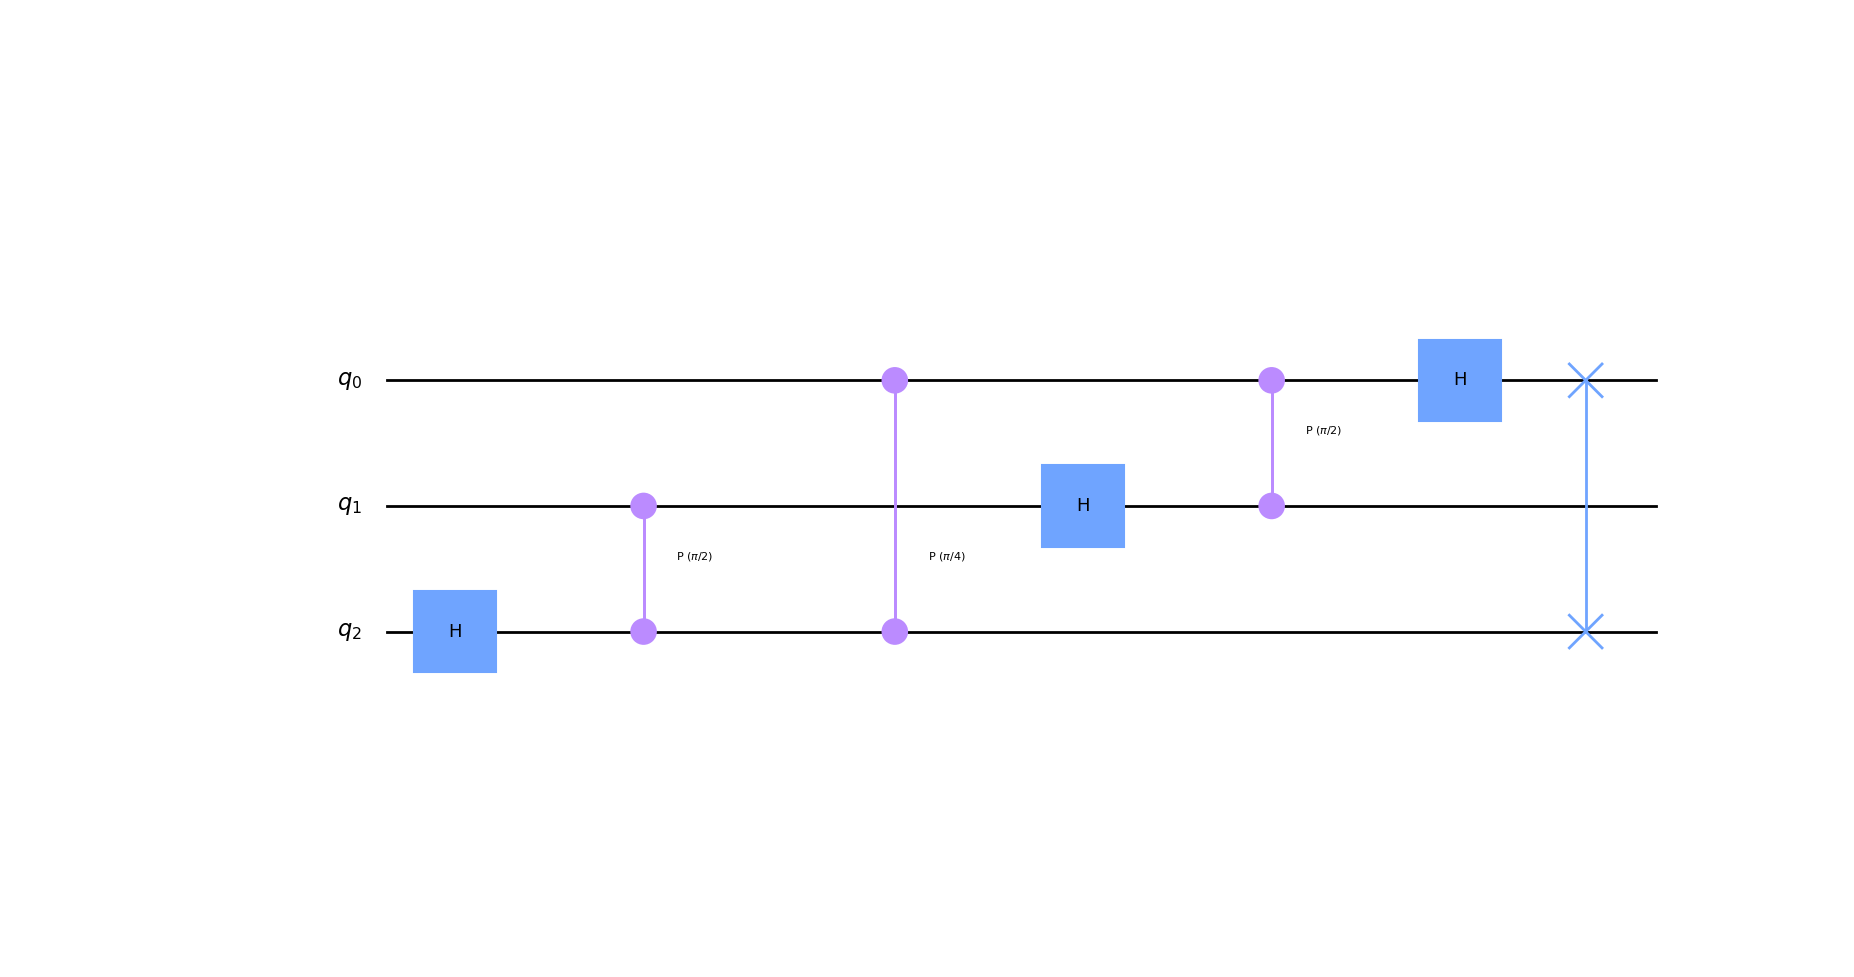
\includegraphics[scale=0.5, center]{./qft_3_qubits.png}
\caption{QFT circuit implementation for three qubits.}
\label{fig::QFT_circuit_3qubits}
\end{figure}

\subsubsection{QFT for n Qubits}
To apply the general transform to $n$ qubits, the previous approach is used together with a programming technique: recursion. The gates are applied to the most significant qubit, and then the same function is called recursively to apply the necessary gates to the next most significant qubit, and so on until all qubits in the circuit have been operated on. To see the sequential circuit diagram, the function was called for $6$ qubits. The result is the following.

\begin{figure}[h]
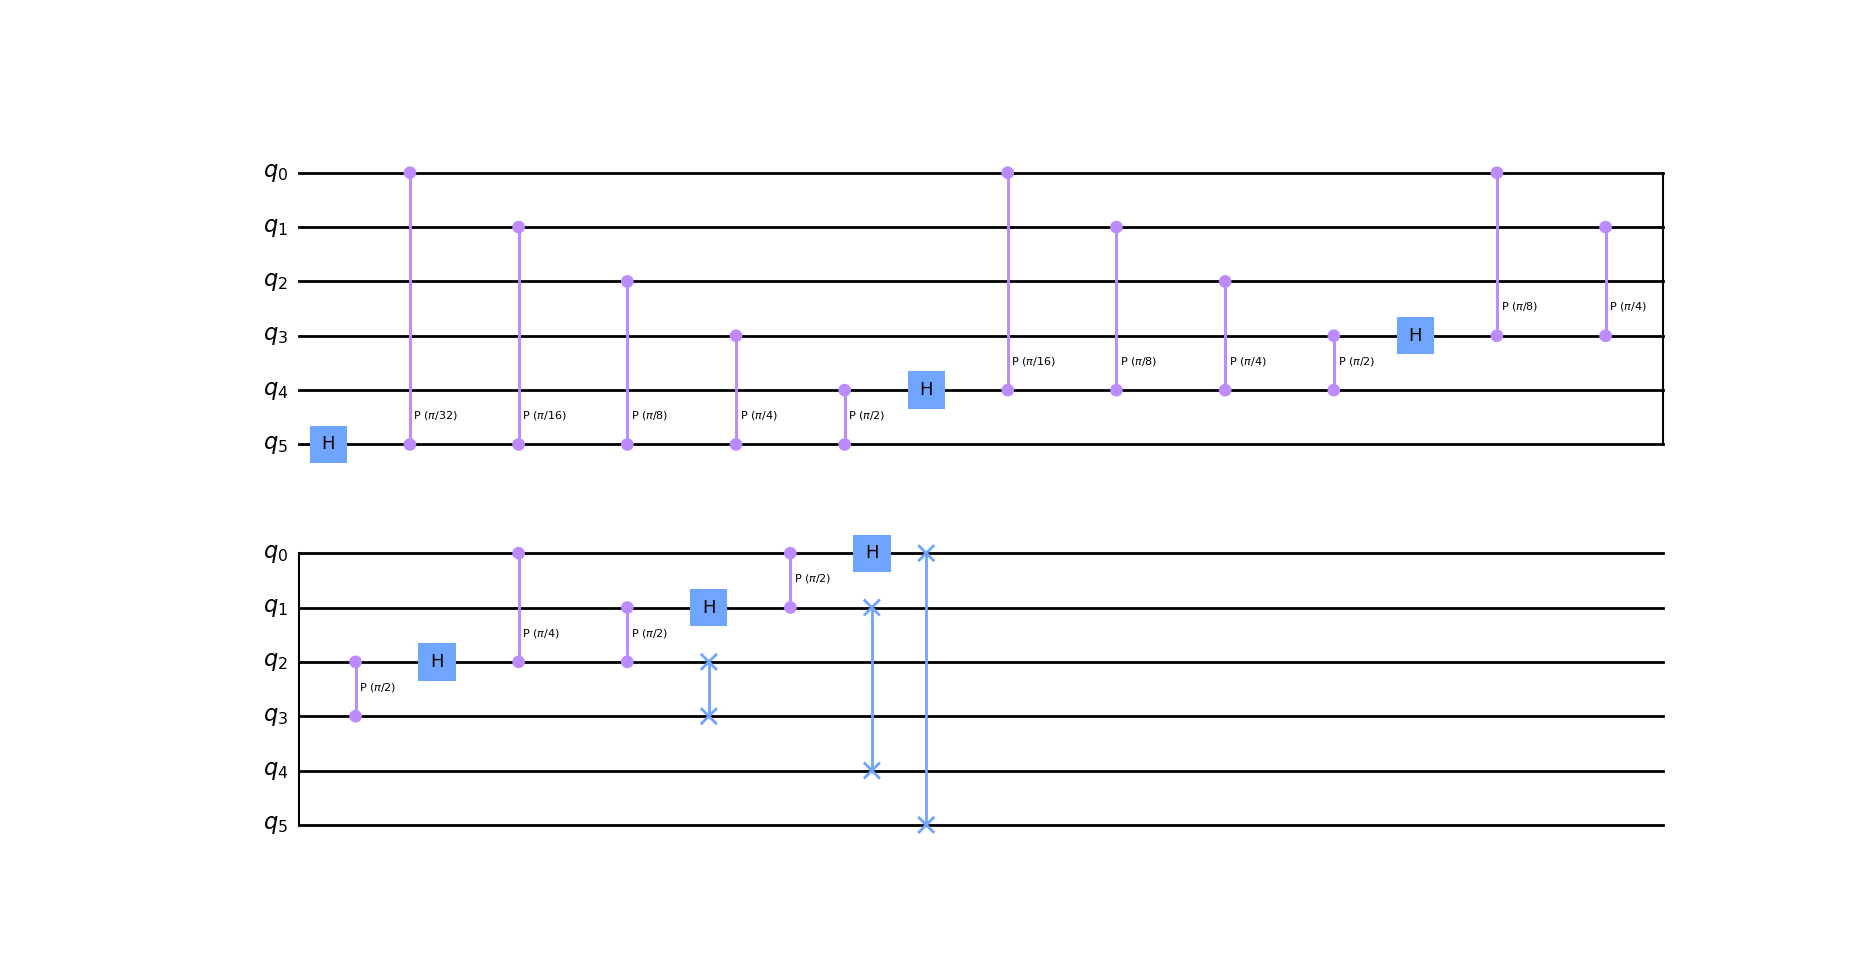
\includegraphics[scale=0.5, center]{./qft_6_qubits.png}
\caption{QFT circuit implementation for six qubits.}
\label{fig::QFT_circuit_6qubits}
\end{figure}
The previous implementations can be found in the GitHub repository: \url{https://github.com/Julio-Medina/Quantum-Fourier-Transform}

\begin{thebibliography}{99}
\bibitem{Arfken} George Arfken. \textit{Mathematical Methods for Physicists}.

\bibitem{Bell} J.S. Bell. \textit{On the Einstein Podolski Rosen Paradox}. \url{https://cds.cern.ch/record/111654/files/vol1p195-200_001.pdf}

\bibitem{Feynman} Richard P. Feynman. \textit{Simulating Physics with Computers}. \url{https://doi.org/10.1007/BF02650179}.

\bibitem{Medina} J. Medina. \textit{Seminar 1 Report: Quantum Computing}. \url{https://github.com/Julio-Medina/Seminario/blob/main/Reporte_final/reporte_final.pdf}

\bibitem{Mermin} N. David Mermin. \textit{Quantum Computer Science: An Introduction}. Cambridge University Press, 2007.

\bibitem{Nielsen} Michael A. Nielsen and Isaac L. Chuang. \textit{Quantum Computation and Quantum Information}. Cambridge University Press, 2010. 10th Anniversary Edition.

\bibitem{Sakurai} J.J. Sakurai. \textit{Modern Quantum Mechanics}. The Benjamin/Cummings Publishing Company, 1985.

\bibitem{Shor} Peter W. Shor. \textit{Algorithms for quantum computation: discrete logarithms and factoring}. Proceedings 35th Annual Symposium on Foundations of Computer Science, 1994.

\bibitem{Qiskit} \textit{Qiskit Textbook}. \url{https://qiskit.org/textbook-beta}

\bibitem{openQASM} OpenQASM. \url{https://github.com/openqasm/openqasm}.
\end{thebibliography}
\end{document}
